\section{\scshape Implémentation}
\subsection*{Implémentation}
\begin{frame}{Implémentation}
	Plusieurs aspects : 
	
	\begin{itemize}
		\itemar Implémentation des algorithmes sur réseaux de Petri.
		\itemar Tests.
		\itemar Implémentation dans le logiciel i-score.
		\itemar Portage sur plate-formes embarquées.
	\end{itemize}
	
	L'implémentation dans le logiciel doit offrir des abstractions simples pour les compositeurs.
	
	\begin{itemize}
		\itemar Création d'abstractions de haut-niveau travaillant avec l'\textsc{API Score} : Session, Groupe, Client, Permission.
	\end{itemize}
\end{frame}

\subsection{Logiciel de test}
\begin{frame}{Logiciel de test}
	\begin{itemize}
		\itemar Simulation de l'exécution d'un réseau de Petri quelconque sur plusieurs machines.
		\itemar Répartition à la volée.
		\itemar Communication par messages \textsc{OSC}.
		\itemar Sert de chantier d'expérimentation pour les choix effectués par la suite.
		\itemar A été porté sur \textsc{Android} pour permettre l'étude de cas réels.
	\end{itemize}
\end{frame}

\subsection{API OSSIA}
\begin{frame}{Implémentation dans l'API OSSIA}
	Permet l'utilisation pour la version en développement de i-score, et depuis le code, ce qui rend possible le développement d'autres logiciels ou d'autres implémentations.
	
	La répartition est faite au niveau du scénario.
	
	Concepts : 
	\begin{itemize}
		\item \textbf{Session}: Rassemble les informations concernant le scénario et les clients connectés. 
		\item \textbf{Client} :  Représente une machine sur le réseau.
		\item \textbf{Groupe} :  Associe des scénarios entre eux, et permet duplication et déplacement.
		\item \textbf{Permission} :  
		Permet des optimisations au niveau de l'envoi de messages entre clients.
	\end{itemize}
\end{frame}

\begin{frame}{Example réparti dans le formalisme OSSIA}
	\begin{figure}
		\centering
		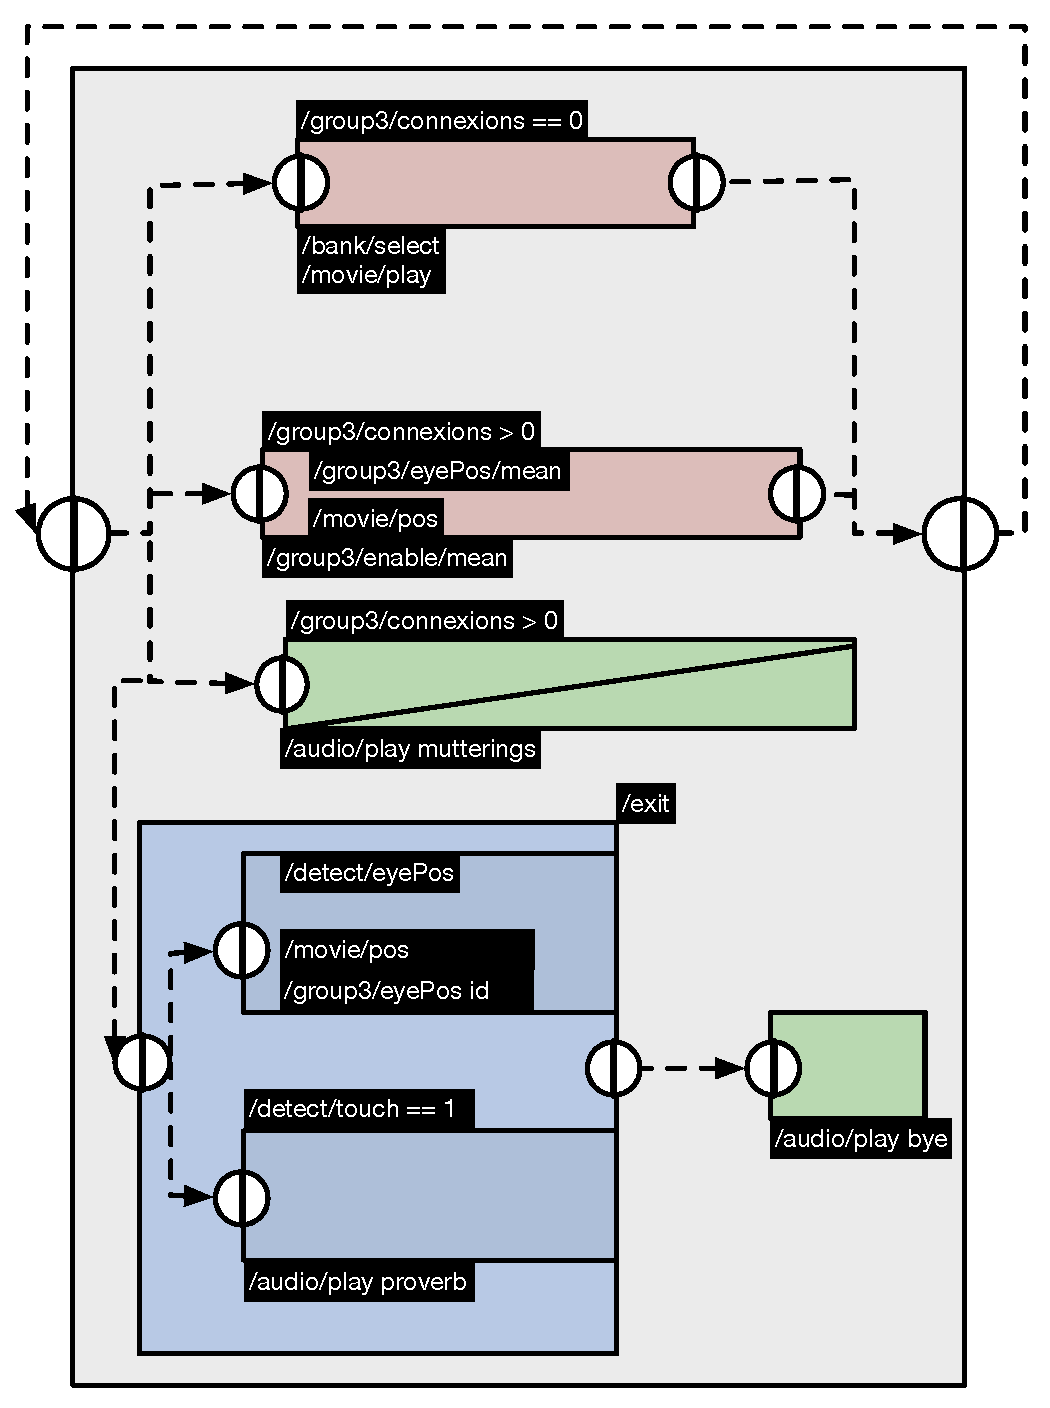
\includegraphics[scale=0.33]{../src/images/ossiaDistri.pdf}
	\end{figure}
\end{frame}

\subsection{Résultats}
\begin{frame}{Résultats}
	Deux protocoles : 
	
	\begin{itemize}
		\item Un en utilisant des machines virtuelles séparées avec une latence quasiment fixe (avec \textsc{WANem}).
		\item Un en utilisant des machines réelles connectées en Wi-Fi.
	\end{itemize}
	
	Résultats obtenus (retard après déplacement d'un segment, sans modification au réseau, puis avec application de la seconde méthode de déplacement présentée précédemment) :

\begin{table}[H]
	\centering
	\tabulinesep=3pt
	\begin{tabu} to \linewidth {XXX}
		Protocole & Sans déplacement & Avec déplacement \\
		\toprule[0.15em]
		VM & $\num{111}\si{\milli\second}$ & $\num{47}\si{\milli\second}$ \\
		Tablettes & $\num{56}\si{\milli\second}$ & $\num{4}\si{\milli\second}$ \\
	\end{tabu}
\end{table}

\end{frame}

